\section{Grid design}
\citet{bertoni:2002} states that the concept of minimalist architecture is to strip everything down to its essential quality and achieve simplicity. The design of the application was to follow this simple rule. The bare essentials were the only aspects that needed to be displayed the user. The set up of the website is to have three blocks displayed in the centre of the screen, laid out on a six column grid. Grid design is important in web design as it add continuity to each page. Each page will have the relevant information in a similar position to the last, allowing the user to be able to extract the information more quickly. A grid layout also makes it easier to design for other devices. \citet{walkers:2013} found that their mobile traffic was up to 29\% in Q2 2013. From this, we can see that more and more people are browsing the internet from the mobile devices. 43\% of this traffic was from iPhones. As web designers, we need to make sure that our web applications looks as good on a 320 pixel width devices as it does on a laptop monitor. This lead to the design of the application being based on a six column grid. This was for two main reasons: the first reason to keep consistency through the sizing of different areas of the website and the second being it makes it much easier to scale the design down for mobile traffic. Due to the fact that mobile traffic is increasing, and also that the application will mainly be used on mobiles, responsiveness was very important when designing the application. It need to have the same feel on a 1920px screen as it would on a 320px mobile device screen.\\

\section{Wireframe and mock up}
Simple designs were sketched up in a notebook to get a feel for how each of the pages would look on both a normal monitor and a mobile devices. After sketches were complete, they were then drawn up in Sketch \citep{sketch:2013} where colour, text, and images can be added to get an even better feel for how the application is going to look and work. Once colour could be applied to the design, user accessability could be thought about. Around 8\% of men in the United Kingdom are affected by some form of colour blindness and 0.5\% of women \citep{colourBlind}. If the design was not to cater for their needs then that would be a percentage of the population that cannot use the application. Colour should never be the primary cue for information. During the design process, changes were made so that any occurrence where colour was the primary cue would also have a visual cue. For example: when the user checks off a goal, the text will have a strike through it as well as turning red. Also, a large percentage of the population have a visual impairment. A few steps were taken to keep the site safe for the visually impaired. The font size and weight is kept at a easy to read level so that it is not taking up to much space but still easily readable. Also, the colour of the font has to contrast with that of its background. From a previous design, the background of the cards and headers was very light and the font colour was too light which would be quite difficult to read for a visually impaired person. Since then, the background colour has completely changed to a darker blue and the colour of the text has been made a lighter shade of grey. As for the typeface, I went with Helvetica, as san-serif fonts are easier to read for the visually impaired. Where there is any large amount of text that the user will need to read, a line height of 1.5 will be used to make it easier to read for visually impaired people. Also, using ARIA HTML5 landmarks, such as header, footer and nav tags, will increase the usability of my website on screen readers. It is important when writing any web application to use semantic HTML that can be used easily without loading the stylesheet file.\\

\begin{figure}[!ht]
\centering
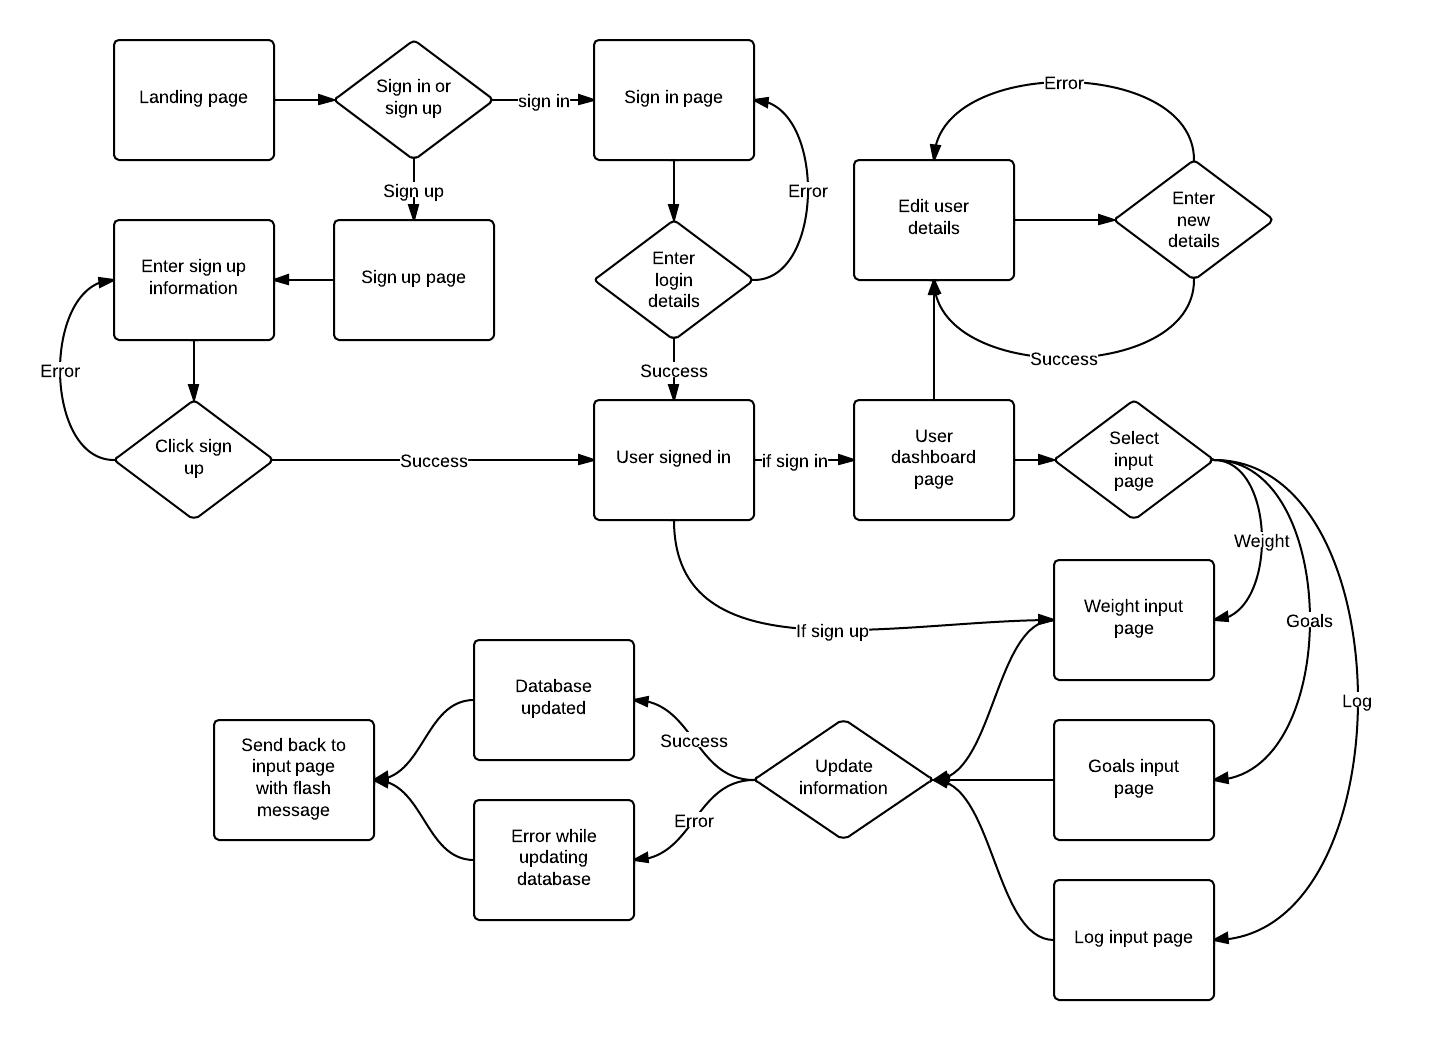
\includegraphics[scale=0.2]{chapters/figs/flowchart}
\caption{Flowchart for the processes and actions of the web application recur.}
\label{fig:flowchart}
\end{figure}

\section{Design in the browser}
Most of the design for the application was drawn up, but some of the easier designs were made directly in the browser. This was to speed up the process by cutting out unnecessary tasks. As opposed to the original plan, development begin during the design stage. This was because there was enough of a design to begin developing some of the application. Once development was underway some things had not been designed yet, for examples; the forms for signing in and out. There was a clear vision of what the forms should look like, so instead of wasting time making the wireframe and mock up of them, they were just designed on the fly, in the browser. This allows for rapid prototyping of the applications looks and lessens the work load on the design front, and even if the design does not work there is no reason why another design cannot be drawn up and implemented.\\

\section{Database design}
As well as design the application, the design of the backend will need to be done before development takes place. For the backend, Ruby on Rails \citep{rails:2013} will be used. Reasons for this will be discussed in the development chapter \ref{dev} page \pageref{dev}. A number of attributes will be store about the user and will be split up over a number of tables all with a one to many relationship to the user table. The other tables will be current weight, which will store the current weight of the user, goal weight, which will store the goal weight of the user, fitness log, which will store information about what exercises they did and how they did, and the goals table, which will store the users goals. All of these will link back to the users ID. Originally, there was going to be a user?s weight table, which store both the current and goal weight but it was moved to two different tables because it is unlikely that the user will be updating the goal weight as much as they were going to update their current weight. All of these tables will have depend upon their user, so if the user is removed from the database so will all their data. Below (Figure \ref{fig:erd}) you can see the entity relationship diagram for the application.

\begin{figure}[!ht]
\centering
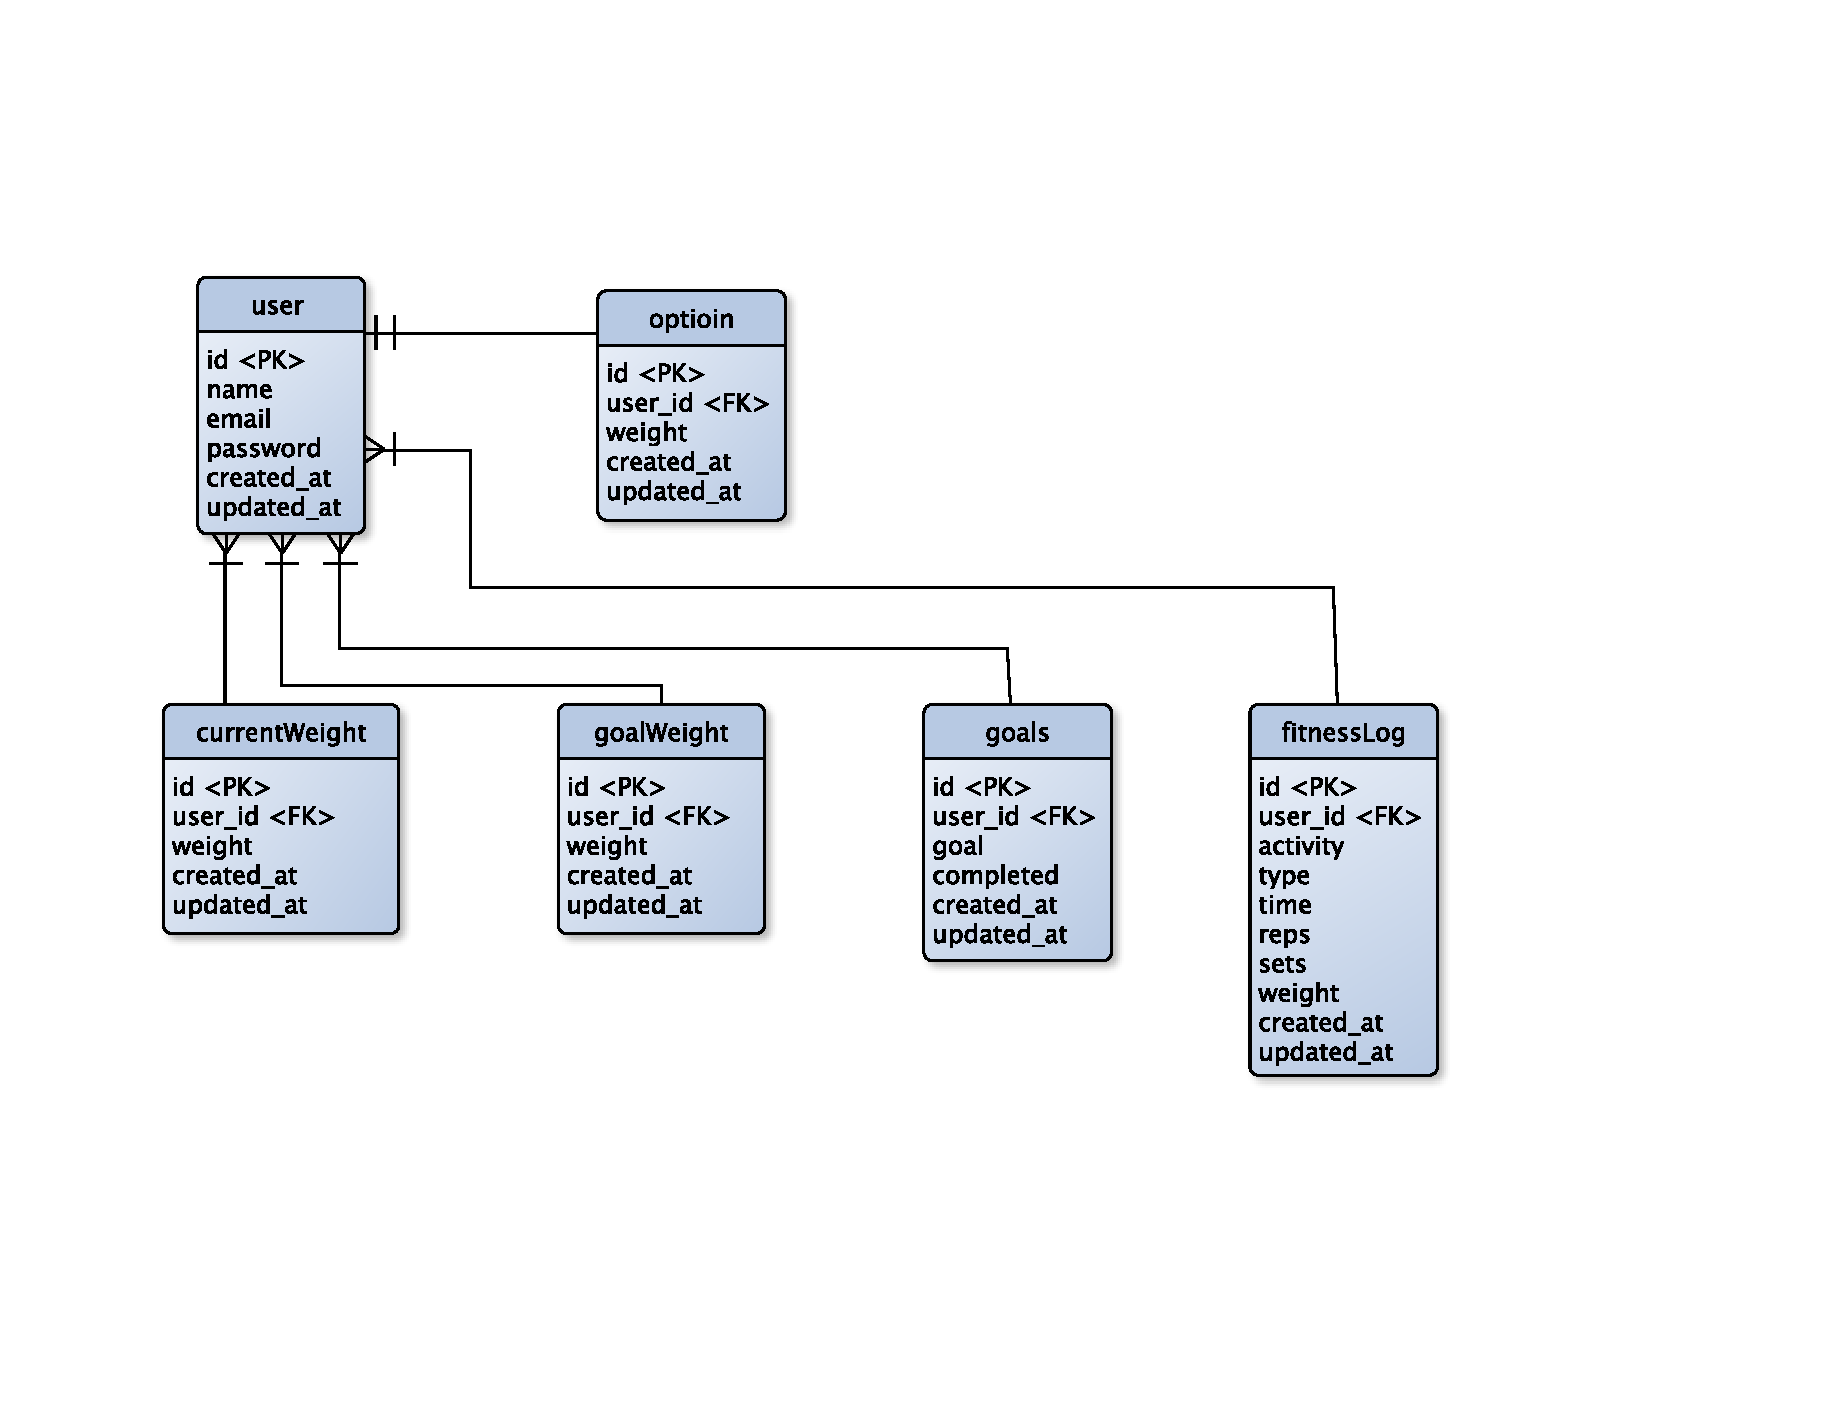
\includegraphics[scale=0.5]{chapters/figs/erd}
\caption{Entity Relationship Diagram for the website application recur.}
\label{fig:erd}
\end{figure}